\chapter{Polarization across Dielectric Interface}\label{lec:lec33}
In the previous chapters, we have been investigating the behaviour of uniform plane waves across a dielectric media interface. We studied two cases which are the parallel and perpendicular polarization, and we saw the transmission and reflection across the dielectric boundary. We also investigated a special case called total internal reflection across a dielectric boundary. Now we are going to discuss another important aspect of electromagnetic waves called the \textbf{Polarization across dielectric interface}. 

We consider a wave which is arbitrarily polarized i.e. the electric field vector makes an arbitrary angle with the plane of incidence and might also be varying as a function of time. We then see how the polarization changes when the wave is reflected from the dielectric interface. So what we are going to investigate now is that, if the incoming wave is coming with a certain polarization, what will be the polarization of the reflected wave and what will also be the polarization of the transmitted wave?

As we have seen earlier, any arbitrary state of polarization can be decomposed into two orthogonal polarizations. Similarly, in this case, we take two linear orthogonal polarizations. One is parallel to the plane of incidence and the other is perpendicular to the plane of incidence. This implies that when the wave is incident on the media interface, the electric field \textbf{$\bar{E}$} can be decomposed into \textbf{E}$_\parallel$\footnote{
Parallel component of the polarized wave
} and \textbf{E}$_\perp$\footnote{
The vertical component of the polarized wave
} with a phase difference of e$^{j\phi}$ between \textbf{E}$_\parallel$ and \textbf{E}$_\perp$.

So the polarized wave will be; $$\textbf{E} = \textbf{E}_\parallel + \textbf{E}_\perp.e^{j\phi}$$	

\section{Decomposition of Polarized wave}	
When an incident polarized wave \textbf{E$_i$} hits a dielectric media interface, part of it gets transmitted through the media(\textbf{E$_t$}), while the other part gets reflected( \textbf{E$_r$}). Each of the fields of the wave i.e. \textbf{E$_i$}, \textbf{E$_t$} and \textbf{E$_r$} can be decomposed into their orthogonal components as explained above.	
\subsection{Incident wave}	
An incident polarized wave \textbf{E$_i$} can be decomposed into two orthogonal components as shown in equation~\ref{equation1_Lec33}	
\begin{equation}
\textbf{E}_i = \textbf{E}_{i\parallel} + \textbf{E}_{i\perp} e^{j\phi}
\label{equation1_Lec33}
\end{equation}
figure~\ref{fig:mcben} shows the two orthogonal components.	
\subsection{Reflected Wave}
Similarly, a reflected polarized wave \textbf{E$_r$} can be decomposed into two orthogonal components as shown in figure~\ref{fig:mcben1}. It can be represented in terms of reflection coefficient as shown in figure~\ref{fig:mcben2}
\begin{equation}
\textbf{E}_r = \textbf{E}_{r\parallel} + \textbf{E}_{r\perp} e^{j\phi}
\end{equation}	
\begin{equation}
\textbf{E}_r = \Gamma_\parallel \textbf{E}_{i\parallel} + \Gamma_\perp \textbf{E}_{i\perp} e^{j\phi}
\end{equation}	
figure~\ref{fig:mcben} shows the two orthogonal components.

\subsection{Transmitted Wave}
A transmitted polarized wave \textbf{E$_t$} can be decomposed into two orthogonal components as shown in equation~\ref{eqn:equation4_Lec33}
\begin{equation}
\textbf{E}_t = \textbf{E}_{t\parallel} + \textbf{E}_{t\perp} e^{j\phi}
\label{eqn:equation4_Lec33}
\end{equation}
It can be represented in terms of the transmission coefficient;	
\begin{equation}
\textbf{E}_t = \tau_\parallel \textbf{E}_{i\parallel} + \tau_\perp\textbf{E}_{i\perp} e^{j\phi}
\end{equation}	
figure~\ref{fig:mcben} shows the two orthogonal components.	

\subsection{Combination of \textbf{E$_i$}, \textbf{E$_r$} and \textbf{E$_t$}}
In combining the incident wave \textbf{E$_i$}, reflected wave \textbf{E$_r$} and transmitted wave \textbf{E$_t$}, we will get a wave structure as that shown in figure~\ref{fig:mcben}	
\begin{figure}[h]
\centering
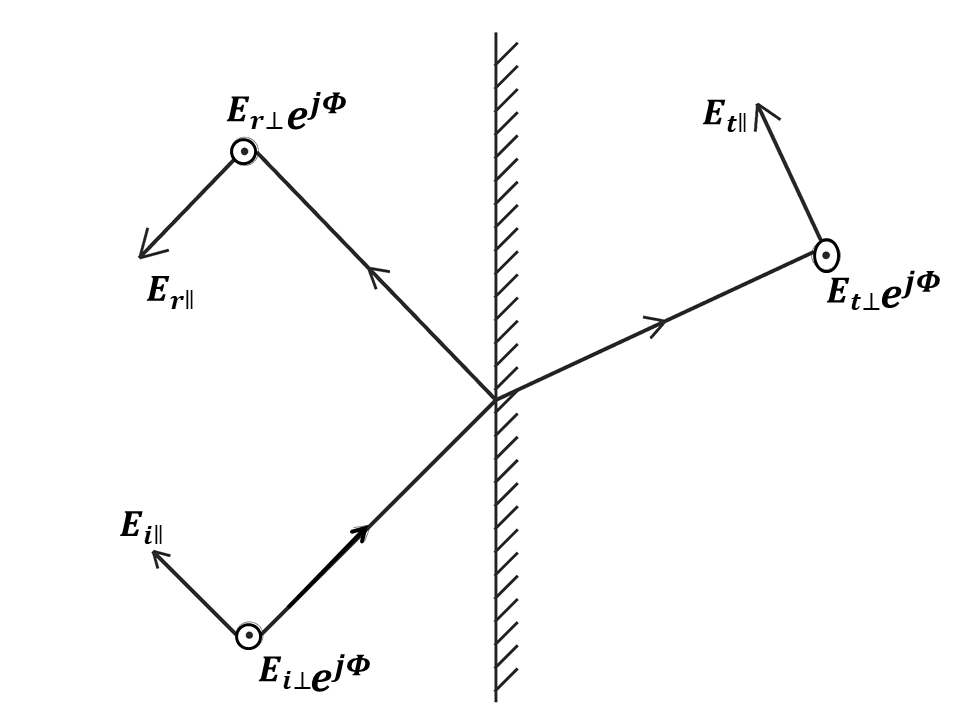
\includegraphics[width=1\linewidth]{\pathtopartone/graphics/orthogonal_components}
\caption{Combination of \textbf{E$_i$}, \textbf{E$_r$} and \textbf{E$_t$}}
\label{fig:mcben}
\end{figure}

Depending on whether it is a normal reflection or total internal reflection, $\tau$ and $\Gamma$ could be real or complex quantities. For normal reflection, $\tau$ and $\Gamma$ are real quantities that can have positive or negative values. However, for total internal reflection, $\tau$ and $\Gamma$ become complex with a magnitude of one. Now we have various possibilities for special cases which we shall discuss in the next section as we may be curious to know what happens to the polarization if the wave was linearly polarized and the reflections were normal or a case of total internal reflection, or perhaps what happens if the wave was circularly polarized.

\section{Linearly Polarized Wave}
In a linearly polarized wave, the electric field vector does not change direction as a function of time. That is, the incident electric field vector makes an angle with the plane of incidence, but its direction remains the same irrespective of time. And as we know, a linearly polarized wave can be decomposed into two components that are orthogonal with no phase difference. So if the wave is linearly polarized, the phase difference between \textbf{E}$_{i\parallel}$ and \textbf{E}$_{i\perp}$ is zero. Hence for this case $\phi$ = 0. We shall now investigate what will happen in the case of normal reflection and also in the case of total internal reflection.

\subsection{Normal Reflection}
Recall that for normal reflection, $\Gamma_\parallel$ and $\Gamma_\perp$ are real. So if $\Gamma_\parallel$ and $\Gamma_\perp$ are real and $\phi$ = 0, then \textbf{E}$_{i\parallel}$ and \textbf{E}$_{i\perp}$ will have a phase of $0$ or $\pi$ radians between them, depending upon the direction of the electric field. In both cases of 0 or $\pi$ phase difference, the polarization remains linear since $\pi$ radians phase shift means a reversal of the electric field. So the orientation of the electric field will change but the polarization will remain linear. So in general, $\Gamma_\parallel \neq \Gamma_\perp$. Hence, a linearly polarized wave will remain linearly polarized since the phase difference is unchanged, but the relative amplitude for the reflected waves might change depending upon whether the condition $\Gamma_\parallel \neq \Gamma_\perp$ is meant or in some special cases where $\Gamma_\parallel$ = $\Gamma_\perp$. This implies that the ratio of both components of the reflected wave will not be the same as it was for the incident wave thus, the direction of the electric field vector is changed for the reflected wave but the wave will remain linearly polarized. So the plane of polarization might change depending upon whether $\Gamma_\parallel$ and $\Gamma_\perp$ are equal or not, but the linearly polarized nature of the wave will be maintained.

\subsection{Total Internal Reflection}
On the other hand, if we have total internal reflection, then $\Gamma_\parallel$ and $\Gamma_\perp$ become complex, but $|\Gamma_\parallel|$ = $|\Gamma_\perp|$ = 1. So the phase difference between $\Gamma_\parallel$ and $\Gamma_\perp$ component in the reflected wave will change as $\Gamma_\parallel$ \textbf{E}$_{i\parallel}$ will have its phase and $\Gamma_\perp$ \textbf{E}$_{i\perp}$ e$^{j\phi}$ will have its own phase. So here the phase difference could be arbitrary which means we would have a linear polarization changing to an elliptic polarization, for the case of total internal reflection. The same thing also applies to the transmitted wave. 

Hence for normal reflection, a linearly polarized wave remains linearly polarized whereas for total internal reflection, a linearly polarized wave becomes elliptically polarized.

\section{Circular Polarization}
Now if the incident wave is circularly polarized, what happens to the transmitted and reflected waves at normal reflections and total internal reflection?

For circular polarization, $\mid$\textbf{E$_r$$_\parallel$}$\mid$ = $\mid$\textbf{E$_r$$_\perp$}$\mid$ and the phase difference between them is $\pm\frac{\pi}{2}$. So $\phi$ = $\pm\frac{\pi}{2}$.

\subsection{Normal Reflection}
Again under  normal reflection, $\mid\Gamma_\parallel\mid \neq \mid\Gamma_\perp\mid$ but $\Gamma_\parallel$ and $\Gamma_\perp$ are real quantities. That means the phase difference between the reflected wave remains $\phi$ = $\pm\frac{\pi}{2}$ but the amplitude ratio for the reflected wave for perpendicular and parallel are not equal because $\mid\Gamma_\parallel\mid \neq \mid \Gamma_\perp \mid$. So $\mid$ \textbf{E}$_{r\parallel} \mid \neq \mid$ \textbf{E}$_{r\perp\mid}$ and the phase difference between the two remains $\pm\frac{\pi}{2}$. Now, the vector sum in this case with varying amplitude gives an elliptical polarization but, the major and minor axis align with the coordinate axis for the ellipse. So the incidence wave was circularly polarized but the reflected wave became elliptically polarized. Since the phase difference between these reflected waves remains $\pm\frac{\pi}{2}$, the major and minor axis of the reflected wave ellipse will lie in the plane of incidence and perpendicular to the plane of incidence respectively or vice versa but the angle which the major axis makes with the plane of incidence could be either zero or $\frac{\pi}{2}$ so the tilt angle for the ellipse with respect to the plane of incidence is either 0 or $\frac{\pi}{2}$.

\subsection{Total Internal Reflection}
With total internal reflection, $\mid\Gamma_\parallel\mid$ = $\mid\Gamma_\perp\mid$ = 1 but $\Gamma_\parallel$ and $\Gamma_\perp$ are complex quantities, meaning
\textbf{E}$_{r\parallel}$ and \textbf{E}$_{r\perp}$ will have same amplitude with \textbf{E}$_{i\parallel}$ and \textbf{E}$_{i\perp}$ respectively but with different phase which is arbitrary. So we get a wave once again that is elliptically polarized.

In summary, a circularly polarized wave under normal reflection gives a reflected wave with elliptical polarization with its major axis at 0 or $\dfrac{\pi}{2}$ to the plane of incidence (tilt angle) and under total internal reflection, a circularly polarized incident wave, in general, gives an elliptically polarized reflected wave.

So in general, we can draw the conclusion that, for an incident wave which is elliptically polarized, the state of polarization of the reflected wave will change depending upon the medium parameters. Hence, an elliptically polarized wave can become circularly polarized or linearly polarized depending upon the medium.

Essentially the important point we have to note from this discussion is that the media interface can be used to alter the state of polarization of an electromagnetic wave. So if we have a certain state of polarization for the incoming wave, then by launching the wave at an arbitrary angle, we should be able to change the polarization to a desired state.

One of the special cases of this is that if the incident wave is some arbitrarily polarized wave, it is possible to make the reflected wave linearly polarized. There are many applications where we require a linearly polarized wave. The source we might have may not generate physically a linearly polarized wave.  So we look for some mechanism by which an arbitrarily polarized wave can be converted into a linearly polarized wave as we saw that the dielectric interface can change the polarization of the electromagnetic wave.

\section{Brewster Angle}
We recall from earlier sections that 
\begin{equation}
\Gamma_\parallel = \dfrac{\eta_1\cos\textit{$\theta$i} - \eta_2\cos\textit{$\theta$t}}  {\eta_1\cos\textit{$\theta$i} - \eta_2\cos\textit{$\theta$t}}
\end{equation}
\begin{equation}
\tau_\parallel = \dfrac{2\eta_2\cos\textit{$\theta$i}} {\eta_1\cos\textit{$\theta$i} + \eta_2\cos\textit{$\theta$t}}
\end{equation}
and,
\begin{equation}
\Gamma_\perp = \dfrac{\eta_2\cos\textit{$\theta$i} - \eta_1\cos\textit{$\theta$t}}  {\eta_2\cos\textit{$\theta$i} - \eta_1\cos\textit{$\theta$t}}
\end{equation}
\begin{equation}
\tau_\perp = \dfrac{2\eta_2\cos\textit{$\theta$i}} {\eta_1\cos\textit{$\theta$i} + \eta_2\cos\textit{$\theta$t}}
\end{equation}
If $\eta_1\cos\theta_{\textit{i}}$ - $\eta_2\cos\theta_{\textit{t}}$ = 0  for parallel or $\eta_2\cos\theta_{\textit{i}}$ - $\eta_1\cos\theta_{\textit{t}}$ = 0 for perpendicular polarization i.e $\Gamma$ = 0, then the wave incident on the dielectric interface is completely transmitted to the second medium. That means if we put a perpendicularly polarized wave at an angle $\Gamma_\perp$ = 0, then the perpendicularly polarized wave goes through without reflection. Similarly a parallel polarized wave incident on the medium with the angle at which $\Gamma_{\parallel}$ = 0, the parallel polarized wave passes through and there is no reflection.
Now if we have an arbitrarily polarized wave and launch at an angle which satisfies $\Gamma_\perp$ = 0, only the perpendicularly polarized component goes through. If it launched at an angle at which $\Gamma_\parallel$ = 0 only the parallel component of polarization passes through the media interface. In either case, the reflected wave would have parallel and horizontal polarization for $\Gamma_\parallel$ = 0 and $\Gamma_\perp$ = 0 respectively. In both situations what is transmitted becomes essentially linearly polarized. We have now the interesting case that for a given parameter, we look for the angle at which $\Gamma_\parallel$ or $\Gamma_\perp$ goes to zero. At this angle, one of the polarization is reflected, and a complimentary polarization is transmitted to the second medium. So an arbitrary state of polarization can be converted to linear polarization.

For parallel polarization, $\Gamma_\parallel$ = 0 when $\eta_1\cos\theta$i - $\eta_2\cos\theta$t = 0 or $\eta_1\cos\theta$i = $\eta_2\cos\theta$t. For perpendicular polarization, $\Gamma_\perp$ = 0 i.e $\eta_2\cos\theta$i - $\eta_1\cos\theta$t = 0 or $\eta_2\cos\theta$i = $\eta_1\cos\theta$t. Where $\eta_1$ and $\eta_2$ are the intrinsic impedances of medium 1 and 2 respectively. From Snell's law $\beta_1\sin\theta$i = $\beta_2\sin\theta$t. By doing some algebra, we can solve for the incident angle $\theta_i$ in the case of parallel and perpendicular polarization and the expressions are shown in equation~\ref{equation10_Lec33} and \ref{equation11_Lec33}. 
\begin{equation}
\tan\theta_{B\parallel} = \dfrac{\beta_2}{\eta_2} \Bigg\{ \dfrac{\eta_1 ^2 - \eta_2 ^2}{\beta_2 ^2 - \beta_1 ^2} \Bigg\}^{\dfrac{1}{2}}
\label{equation10_Lec33}
\end{equation}
\begin{equation}
\tan\theta_{B\perp} = \dfrac{\beta_2}{\eta_1} \Bigg\{ \dfrac{\eta_2 ^2 - \eta_1 ^2}{\beta_2 ^2 - \beta_1 ^2} \Bigg\}^{\dfrac{1}{2}}
\label{equation11_Lec33}
\end{equation}

These angles at which the reflection coefficient goes to zero, that is, $\Gamma_\parallel$ = $\Gamma_\perp$ = 0 are called the BREWSTER ANGLE\index{brewster angle}, therefore $\theta_B$ is the Brewster angle. So we have a Brewster angle for parallel and perpendicular polarizations. In general, if we take a medium which could be magnetic, then the Brewster angle for both polarization exists. So at the Brewster angle for parallel polarization, the reflected wave will have only a perpendicularly polarized wave and at the Brewster angle for perpendicular polarization, the reflected wave has only a parallel wave. The Brewster angles for parallel and perpendicular polarization can be derived as follows.

\subsection{Parallel Polarization}
Previously, we derived the relationships below
\begin{dmath}
\eta_1\cos\theta_i = \eta_2\cos\theta_t  = \eta_2\sqrt{1 - \sin^2\theta_t} = \eta_2\sqrt{1- \Bigg\{\dfrac{\beta_1}{\beta_2}\Bigg\}^2\sin^2\theta_i}
\end{dmath}
because $\beta_1\sin\theta_i$ = $\beta_2\sin\theta_t$ from snell's law. so
\begin{equation*}
\beta_2\eta_1\cos\theta_i = \eta_2\sqrt{\beta_2^2-\beta_1^2\sin^2\theta_i}
\end{equation*}
or
\begin{equation}
\cos\theta_i\dfrac{\beta_2\eta_1}{\eta_2} = \sqrt{\beta_2^2-\beta_1^2\sin^2\theta_i}
\label{eqn:equation13_Lec33}
\end{equation}
if we square both sides of equation~\ref{eqn:equation13_Lec33}, we get
\begin{equation*}
\cos^2\theta_i \dfrac{\beta^2_2\eta^2_1}{\eta^2_2} = \beta^2_2 - \beta^2_1\sin^2\theta_i
\end{equation*}
or
\begin{equation}
\dfrac{\beta^2_2\eta^2_1}{\eta^2_2}(1 - \sin^2\theta_i) = \beta^2_2 - \beta^2_1\sin^2\theta_i
\end{equation}
\begin{equation*}
\dfrac{\beta^2_2\eta^2_1 - \beta^2_2\eta^2_2}{\eta^2_2} = (\dfrac{\beta^2_2\eta^2_1}{\eta^2_2} - \beta^2_1)\sin^2\theta_i
\end{equation*}
\begin{equation*}
\beta^2_2\eta^2_1 - \beta^2_2\eta^2_2 = (\beta^2_2\eta^2_1 - \beta^2_1\eta^2_2)\sin^2{\theta_i}
\end{equation*}
\begin{equation}
\sin^2{\theta_i} = \dfrac{\beta^2_2\eta^2_1 - \beta^2_2\eta^2_2}{\beta^2_2\eta^2_1 - \beta^2_1\eta^2_2}
\label{eqn:equation15_Lec33}
\end{equation}
from trigonometry, we have that,
\begin{equation*}
\cos^2{\theta_i} = 1 - \sin^2{\theta_{ii}}
\end{equation*}
so substituting that in equation~\ref{eqn:equation15_Lec33} we get,
\begin{equation}
\cos^2{\theta_i} = 1 - \Bigg\{\ \dfrac{\beta^2_2\eta^2_1 - \beta^2_2\eta^2_2}{\beta^2_2\eta^2_1 - \beta^2_1\eta^2_2} \Bigg\}
\end{equation}
also from trigonometry, we know that
\begin{equation*}
\tan^2\theta_i = \dfrac{\sin^2\theta_i}{\cos^2\theta_i} = \Bigg\{\ \dfrac{\beta^2_2\eta^2_1 - \beta^2_2\eta^2_2}{\beta^2_2\eta^2_1 - \beta^2_1\eta^2_2} \Bigg\} = \Bigg\{\ \dfrac{\beta^2_2\eta^2_2 - \beta^2_2\eta^2_1}{\beta^2_2\eta^2_1 - \beta^2_1\eta^2_2} \Bigg\}
\end{equation*}
replacing $\theta_i$ with $\theta_{B\parallel}$
\begin{equation}
\tan\theta_{B\parallel} = \sqrt{\dfrac{\beta^2_2(\eta^2_1 - \eta^2_2)}{\eta^2_2(\beta^2_2 - \beta^2_1)}} = \dfrac{\beta_2}{\eta_2}\Bigg\{\ \dfrac{\eta^2_1 - \eta^2_2}{\beta^2_2 - \beta^2_1} \Bigg\}^{\frac{1}{2}}
\end{equation}

\subsection{Perpendicular Polarization}
Let's assume that the electric field was perpendicular to the plane of incidence as shown in figure~\ref{fig:mcben1} (Pointing out of the plane of the paper as indicated by the dot). Irrespective of variation in $\theta_i$,  \textbf{E}$_i$ will remain perpendicular to the plane of incidence and its amplitude is fixed. So when the continuity of the electric field is applied, we get a reflected and transmitted field. The sum of \textbf{E}$_i$ and \textbf{E}$_r$ must be equal to \textbf{E}$_t$ i.e. tangential component of the electric field must be continuous across the boundary. The amplitude of \textbf{E}$_i$, \textbf{E}$_r$ and \textbf{E}$_t$ don't depend on lunching angle $\theta_i$. Hence the reflected field \textbf{E}$_r$ will always be needed to satisfy the boundary condition at the interface.
\begin{figure}[h]
\centering
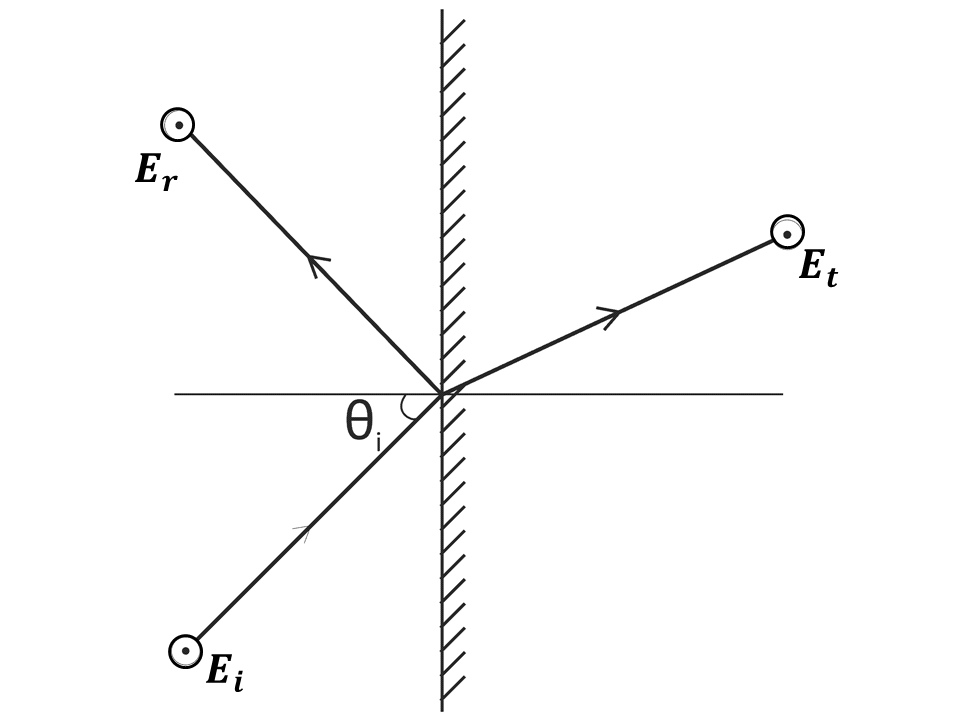
\includegraphics[width=.1\linewidth]{\pathtopartone/graphics/perpendicular_polarization4}
\caption{Perpendicular polarization}
\label{fig:mcben1}
\end{figure}
\begin{figure}[h]
\centering
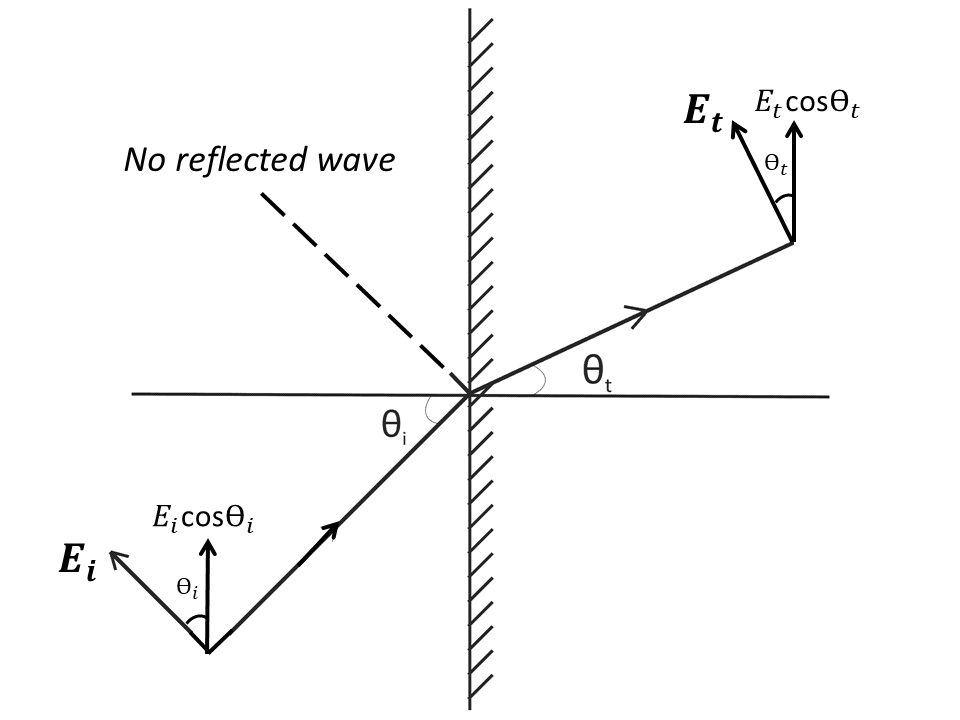
\includegraphics[width=1\linewidth]{\pathtopartone/graphics/No_reflection}
\caption{Parallel polarization}
\label{fig:mcben2}
\end{figure}	

However, for the parallel polarization, variation of $\theta_i$ affects the tangential component of \textbf{E}$_i$ and \textbf{E}$_t$ and they vary with $\theta_i$ as shown in figure~\ref{fig:mcben2}. So there is an angle at which \textbf{E}$_t$ tangential equals \textbf{E}$_i$ tangential i.e \textbf{E}$_i\cos\theta_i$ = \textbf{E}$_t\cos\theta_t$, and then, the electric field due to reflection is not required any more to satisfy the boundary condition. That means \textbf{E}$_r$ will not be needed anymore to satisfy the boundary condition at the interface hence, the reflected wave is absent. So at \textbf{E}$_i\cos\theta_i$ = \textbf{E}$_t\cos\theta_t$, the wave incident is completely transmitted. Since the tangential component varies with the angle of incidence, at some point, there is no reflected electric field required to satisfy the boundary condition.

For perpendicular polarization, this is not the case because the electric field perpendicular to the plane of the paper does not depend on $\theta_i$ and so \textbf{E}$_r$ is always required, so that \textbf{E}$_i$ + \textbf{E}$_r$ = \textbf{E}$_t$. If $\mu_1 \neq \mu_2$ i.e. the media were magnetic, so whatever applies to the electric field applies to the magnetic fields and then we have Brewster angle for perpendicular polarization also. However, for a media which is a pure dielectric, ie $\mu_1 = \mu_2$, then the Brewster angle will only exist for parallel polarization and will not exist for perpendicular polarization.

$\theta_{B\parallel}$ = $\tan^{-1}\left(\sqrt{\dfrac{\epsilon_2}{\epsilon_1}}\right)$ = $\tan^{-1}\left(\dfrac{\eta_2}{\eta_1}\right)$ were $\eta_2$ and $\eta_1$ are the refractive index of medium 2 and medium 1 respectively because $\dfrac{\eta_2}{\eta_1}$ = $\sqrt{\dfrac{\epsilon_2}{\epsilon_1}}$.

Generally, for the dielectric media, we have the Brewster angle for parallel polarization. One can make use of this Brewster angle for converting an arbitrarily polarized wave to a linearly polarized wave. From the diagram below, the incident wave is arbitrarily polarized hence it would have perpendicular and parallel polarized components. At an incidence angle = $\theta_{B\parallel}$, the reflected wave is made out of a purely perpendicular polarized field \textbf{E}$_{r\perp}$ as the parallel polarized reflected wave will not exist. For the transmitted wave , the \textbf{E}$_{i\parallel}$ passes through since incidence angle is $\theta_{B\parallel}$. Some of the perpendicular components will pass through also as $\theta_{B\parallel}$ is not its polarizing angle of $\theta_{B\perp}$.

\begin{figure}[h]
\centering
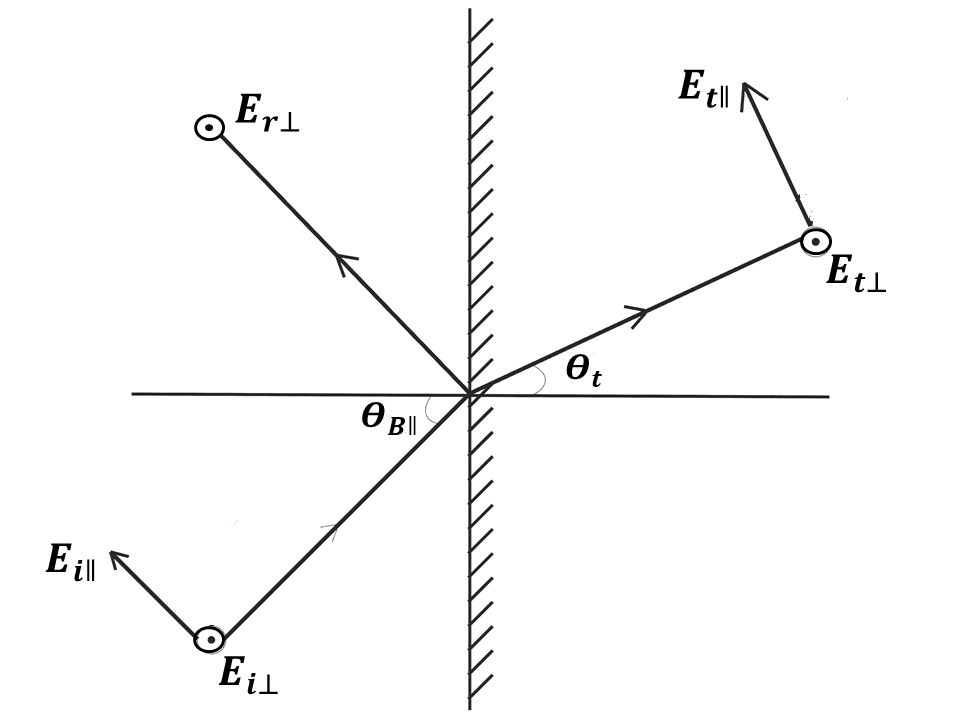
\includegraphics[width=1\linewidth]{\pathtopartone/graphics/No_parallel_reflected_wave}
\caption{}
\label{}
\end{figure}

Hence it is just like a normal wave incident at an angle. So the transmitted wave can in general be elliptically polarized since it has both parallel and perpendicular polarized components.
So without worrying about the state of polarization of the incoming wave, whether linear, circular or elliptically polarized, if the wave is launched at the Brewster angle, then the reflected wave will have a polarization which is linear polarization and its orientation will be perpendicular to the plane of incidence. Hence for any arbitrarily polarized wave incident at the Brewster angle $\theta_{B\parallel}$, the reflected wave \textbf{E}$_{r\perp}$ points outward in the manner shown perpendicular to the plane of incidence. For this reason, $\theta_{B\parallel}$ is also called the \textbf{polarizing angle}. Since a wave launched at that angle has a reflected wave which is linearly polarized. The polarizing angle finds application in polarizing the light beams in lasers, ie if the polarization was arbitrary, we can always use the concept of Brewster angle to make sure the reflected wave is linearly polarized. 

So our conclusion from the discussion is that, by using the dielectric interfaces, one can change the state of polarization of electromagnetic waves. Though this has been shown here for optical beams, for other radio frequencies, one can also make use of this phenomenon for changing the state of polarization of electromagnetic waves.
Later when we talk about reflection and refraction from conducting boundaries, we will consider how the state of polarization would be affected from the incident to the reflected wave.  We have seen for the light incident at Brewster angle, an arbitrary polarization gives a reflected light that is linearly polarized. In conducting boundaries, however, the case is a little simpler and we will observe an interesting phenomenon then. 
So this essentially gives us an idea of how to use dielectric boundaries to change the state of polarization of electromagnetic waves. 

Now suppose we have a general media boundary for which $\sigma_1 \neq \sigma_2 \neq 0$, we may ask, \emph{what happens to the reflected and transmitted wave in this general media?} To solve this problem we first satisfy the boundary conditions at the interface that is, we have to satisfy the boundary condition for the tangential components of the electric and magnetic fields. Even though conductivity is not zero, it is not infinity either so we still do not have a surface current and because of that, we can still apply the boundary conditions which we applied earlier for the dielectric media interface hence, the expressions which we got for $\Gamma_\parallel$, $\Gamma_\perp$, $\tau_\parallel$ and $\tau_\perp$ are still valid.  But the expressions for the intrinsic impedances in both cases $\eta_1$ and $\eta_2$ now becomes $\eta_1$ = $\sqrt{\dfrac{j\omega\mu_1}{\sigma_1 + j\omega\epsilon_1}}$ and $\eta_2$ = $\sqrt{\dfrac{j\omega\mu_2}{\sigma_2 + j\omega\epsilon_2}}$ as we have taken the conductivity into consideration. And because of this, the transmission and reflection coefficients become complex quantities.

So for a general lossy media like this, the analysis is the same with $\eta_1$ and $\eta_2$ appropriately chosen. But with $\gamma$ = $\alpha + j\beta$ being complex in the presence of loss, indicating that there is some attenuation in the system. 

Earlier in our discussion, when a plane wave was incident on a dielectric interface, it did not matter from where the wave originated since the wave amplitude doesn't change even if we travel an infinite distance for a lossless medium. However for a lossy media if we assume that this wave was incident on the boundary at an infinite distance from the surface and $\gamma_1$ = $\alpha_1 + j\beta_1$ ie complex, then the wave amplitude decreases exponentially as it travels. So after travelling an infinite distance, the amplitude which reaches the boundary interface of the lossy media will be zero. Similarly, if we had considered that the wave had a finite amplitude at the interface, coming from an infinite distance as a plane wave, then it should have had an infinite amplitude from the point where the wave originated. So in the case of a lossy medium, it would look as if we require an infinite amount of energy to start with if the wave travels from infinity. This is a hypothetical situation. Without getting into the issue of where the wave originated from, we can assume that when the wave reaches the media interface, it will have a certain amplitude and then the amplitude of the reflected wave just before the interface and the amplitude of the transmitted wave just after the media interface will be given by the reflection and transmission coefficient respectively. 

Now when a wave travels backwards from medium 2 to medium 1, the incident wave amplitude is going to grow exponentially as you move away from the interface further into medium 1. So in medium 2, we have a travelling wave with propagation constant $\gamma_2$ and whose amplitude is exponentially decaying as we move in the direction of travel further into medium 2.

In medium 1, the fields seen are a superposition of the incident and reflected waves. The incidence wave exponentially grows and the reflected wave exponentially decays as we go away from the interface. This case is identical to a lossy transmission line. As we go away from the interface or termination point in a transmission line, the reflected wave becomes weaker and weaker, the transmitted wave grows larger. So essentially as you go away from the interface into medium 1, we see a phenomenon equivalent to that of a travelling wave in a transmission line and when we come close to the boundary, we see some kind of standing wave behaviour. This is identical to what we had seen for a lossy transmission line.

So in conclusion, the analysis of a lossy media interface where the conductivity is finite( it is not 0 or $\infty$), i.e. non of the media is an ideal conductor or dielectric, the problem can still be handled exactly in the same way as we did for the dielectric media interface. We can apply the same boundary conditions and the same expressions for the reflection and transmission coefficients. Then substituting appropriately for the intrinsic impedances for the two media, we can get the expressions for the reflection and transmission coefficients for a lossy media interface. 
